\section{Background}

The shape-and-effect inference system described by Abal et. al. \cite{Abal2017EffectiveBF} enables \begin{quote}
    "[...] efficient and scalable inter-procedural reasoning about resource manipulation"
\end{quote}
 
\newpar Abal et. al. describe a method for detecting double-lock bugs in the kernel source code using the EBA analyzer.

\newpar Extending the approach used by Iago et. al. allows emplying the same shape and effect analysis concepts in addition to the Computational Tree Logic (CTL) problem formulation used in their approach. Furthermore, extending the implementation of their tool allows building an error checker which is already able to run on the Linux kernel components.

\newpar The Linux kernel component source code can be analyzed using existing static analysis tools in order to find a Control Flow Graph (CFG) of a given component implementation. The control flow graph of a given Linux kernel component shows the possible execution paths of the component. These control flow graphs can be formulated in Computational Tree Logic, which in turn allows describing desirable or undesirable execution paths. 

\newpar Iago et. al. formulate the double \textit{lock} error using CTL as: 

\begin{center}
    $\top\:\mathrm{EU}\:\left({l o c k}_{\rho} \wedge\:\mathrm{EX}\:\left(\neg {u n l o c k}_{\rho}\:\mathrm{EU}\:{l o c k}_{\rho}\right)\right)$
\end{center}

\newpar $p$ specifies that I am interested in finding a double lock locking the same memory region, since this is where an infinite spinlock would occur. 

\newpar Computation tree logic is in a class of temporal logics that includes linear temporal logic (LTL), modeling program paths in time as a tree-like structure where all paths can be the actual path executed at runtime. The specifics of the CTL formulation is not the focus of this project, instead CTL notation is merely used to formulate which errors are desired found in the Linux kernel components. CTL be used to model all possible executions of a program avoid some undesirable condition - in this case a double-unlock error.

\newpar This CTL formulation can be visualized in Fig \ref{fig:doublelock}.

\begin{figure}[h]
    \centering
    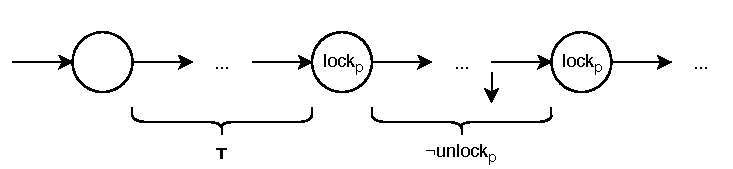
\includegraphics{background/figures/doublelock}
    \caption{The CTL form of a double lock error visualized.}
    \label{fig:doublelock}
\end{figure}

\newpar The inverse problem - the case of two unlocks being present with no locks in between them - can therefore be formulated in CTL as: 

\begin{center}
    $\top\:\mathrm{EU}\:\left({u n l o c k}_{\rho} \wedge\:\mathrm{EX}\:\left(\neg {l o c k}_{\rho}\:\mathrm{EU}\:{u n l o c k}_{\rho}\right)\right)$
\end{center}

\newpar $p$ specifies that I am interested in finding a double unlock locking the same memory region, since this is where the undefined behaviour would occur.

\newpar The visualization of this can be seen in Fig \ref{fig:doubleunlock}.

\begin{figure}[h]
    \centering
    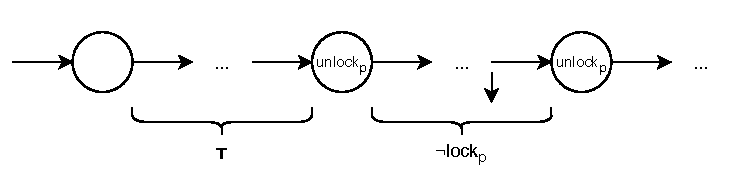
\includegraphics{background/figures/doubleunlock}
    \caption{The CTL form of a double unlock error visualized.}
    \label{fig:doubleunlock}
\end{figure}

\newpar The existing implementation of the EBA analyzer explores the CFG of the Linux kernel components while checking in order to validate that a given undesired execution path is not present in the source code. If such an execution path is found, a bug is possibly present in the analyzed component.

\newpar The implementation of the EBA analyzer uses a concept of \textit{may lock} and \textit{must lock} internally similar to the concept described in \cite{Godefroid}. A lock within an \texttt{if} statement on a dynamic value is represented as a \textit{may lock}, since it is uncertain whether the \texttt{if} statement will evaluate to \texttt{true} at runtime. On the other hand, a \textit{must lock} is an explicit lock within the code which will always be executed. This concept of \textit{may} and \textit{must} also applies to the double unlock problem, where a \textit{may unlock} is an unlock in an execution branch which might not be executed at runtime. A \textit{must unlock} is an explicit unlock where a lock will always be unlocked at runtime.

\newpar The implementation of the EBA analyzer supports implementing separate error checkers in a plug-and-play nature. This allows implementing a double unlock checker as a separate file in the implementation source code and making this available to the user(s) of the analyzer using a command-line parameter. The implementation of my work has been incorporated into the EBA code base in this fashion. The following section will elaborate on the implementation details of this implementation. 